\documentclass[border=10pt]{standalone}

\usepackage{tikz}
\usepackage{tikzsymbols}
\usetikzlibrary{calc,patterns,shapes.geometric}

\def\centerarc[#1](#2)(#3:#4:#5){\draw[#1] ($(#2)+({#5*cos(#3)},{#5*sin(#3)})$) arc (#3:#4:#5);}

\begin{document}
	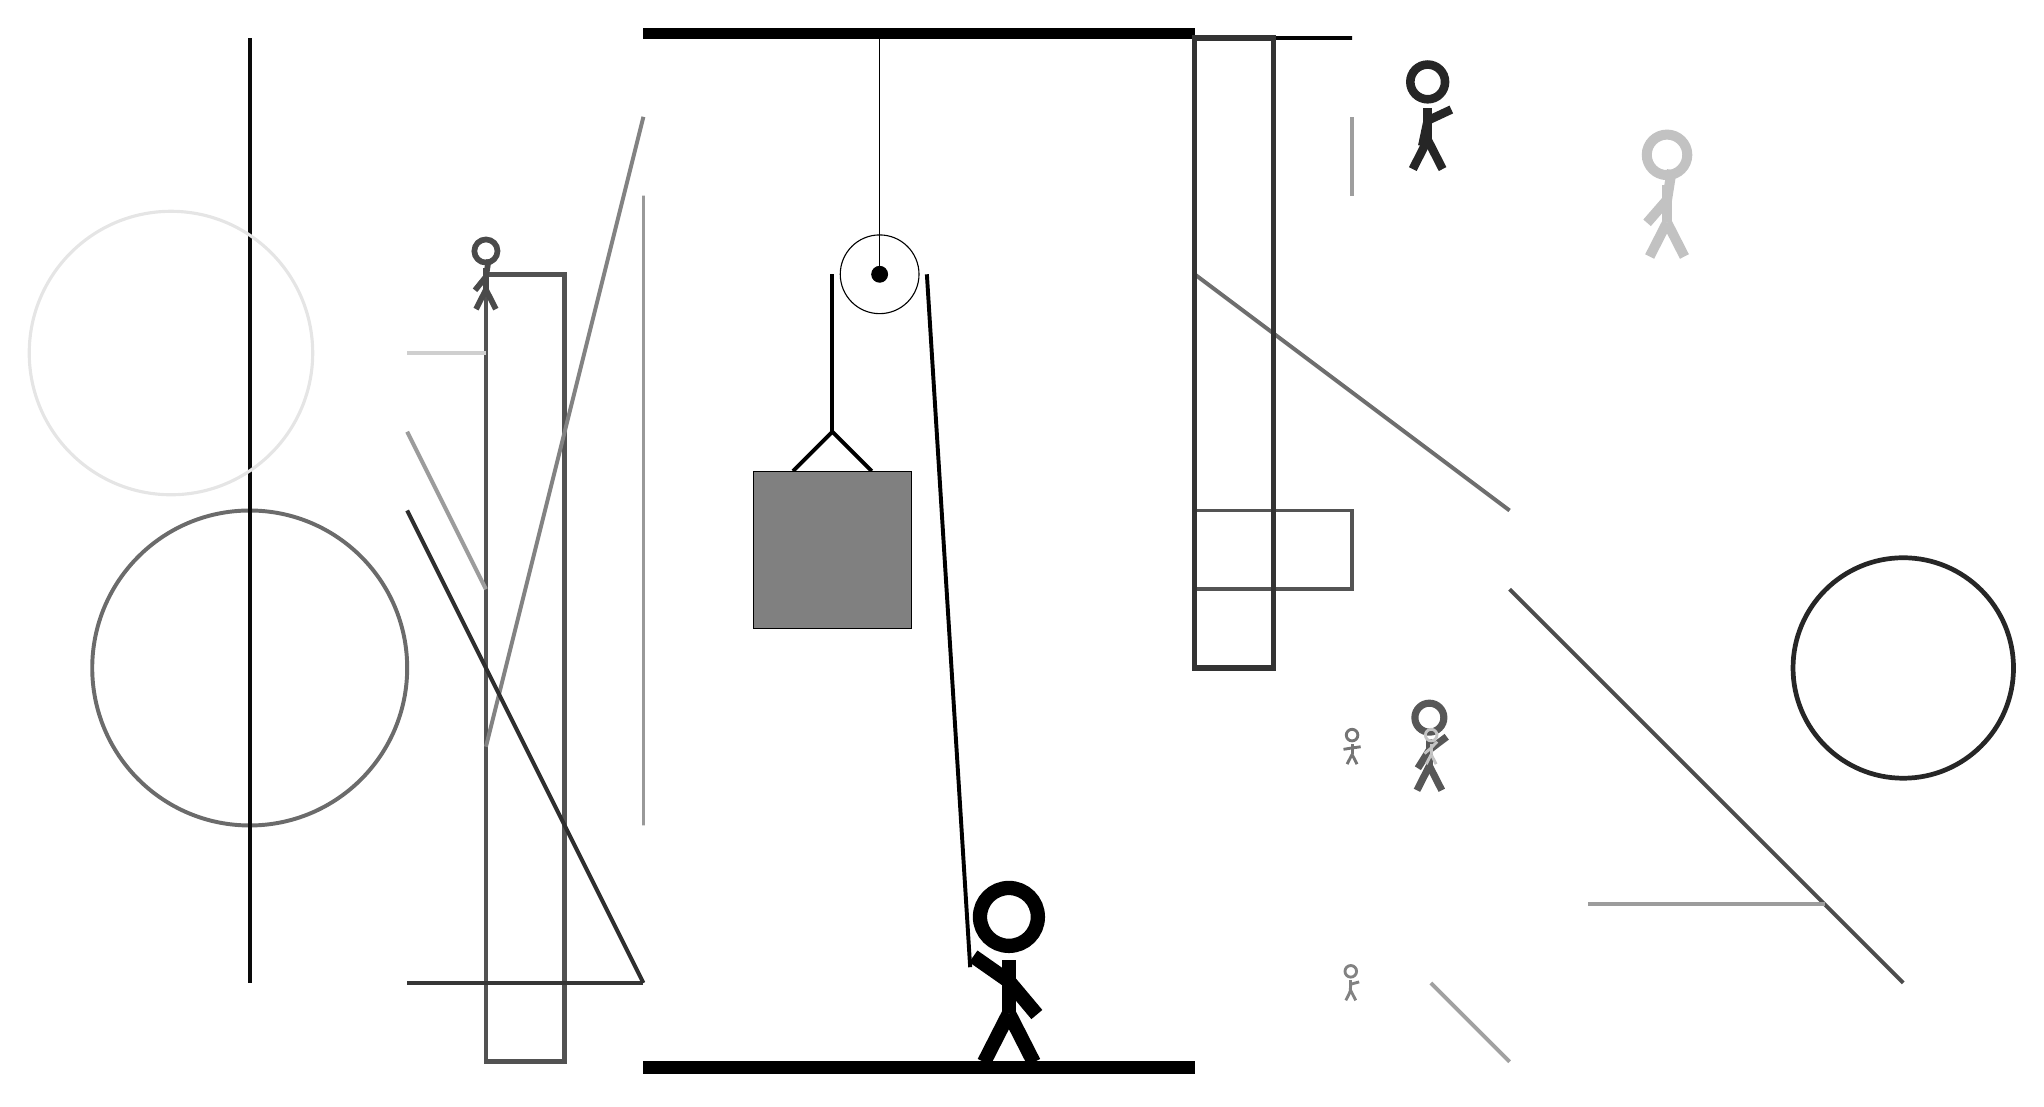
\begin{tikzpicture}
		%%%%% START %%%%%
		
		\draw[fill=black] (-2, 10) rectangle (5, 10.125);
		
		\draw (1, 7) circle (0.5);
		\draw[fill=black] (1, 7) circle (0.1);
		\draw (1, 10) -- (1, 7);
		
		\draw[line width=0.5mm] (-0.1, 4.5) -- (0.4, 5.0) -- (0.9, 4.5);
		\draw[fill=black!50] (-0.6, 4.5) rectangle (1.4, 2.5);
		
		\draw[line width=0.5mm] (0.4, 7) -- (0.4, 5.0);
		\centerarc[line width=0.5mm](1, 7)(0:180:0.6);
		\draw[line width=0.5mm](1.6, 7) -- (2.15, -1.8);
		
		\node at (2.6, -1.9) {\Strichmaxerl[10][-35][-50]};
		
		\draw [line width=0.5mm, color=black!58](-7, 2) circle (2.0);
		
		\draw[line width=0.6mm, color=black!68] (-3, 7) rectangle (-4, -3);
		\node[line width=0.3mm, color=black!49] at (7, -2) {\Strichmaxerl[2][85][15]};
		\node[line width=0.6mm, color=black!66] at (8, 1) {\Strichmaxerl[5][58][37]};
		\draw[line width=0.5mm, color=black!38](7, 8) -- (7, 9);
		
		\draw[line width=0.5mm, color=black!49](-4, 1) -- (-2, 9);
		
		\draw[line width=0.5mm, color=black!99] (5, 10) rectangle (7, 10);
		\draw[line width=0.3mm, color=black!40] (-2, 0) rectangle (-2, 8);
		\draw[line width=0.5mm, color=black!70](9, 3) -- (14, -2);
		\draw[line width=0.5mm, color=black!39](-4, 3) -- (-5, 5);
		
		\draw[line width=0.5mm, color=black!96](-7, -2) -- (-7, 10);
		\draw [line width=0.4mm, color=black!10](-8, 6) circle (1.8);
		\draw[line width=0.5mm, color=black!37](8, -2) -- (9, -3);
		
		\node[line width=0.7mm, color=black!54] at (7, 1) {\Strichmaxerl[2][9][8]};
		\draw[line width=0.5mm, color=black!39](10, -1) -- (13, -1);
		\draw[line width=0.5mm, color=black!67] (7, 3) rectangle (5, 4);
		
		\draw[line width=0.5mm, color=black!79](-5, -2) -- (-2, -2);
		
		\draw[line width=0.5mm, color=black!82](-5, 4) -- (-2, -2);
		\node[line width=0.7mm, color=black!24] at (11, 8) {\Strichmaxerl[7][49][81]};
		\draw[line width=0.5mm, color=black!57](5, 7) -- (9, 4);
		\node[line width=0.2mm, color=black!71] at (-4, 7) {\Strichmaxerl[4][51][81]};
		
		\node[line width=0.5mm, color=black!23] at (8, 1) {\Strichmaxerl[2][40][47]};
		\draw[line width=0.7mm, color=black!80] (5, 10) rectangle (6, 2);
		\draw[line width=0.6mm, color=black!19] (-4, 6) rectangle (-5, 6);
		\draw [line width=0.6mm, color=black!85](14, 2) circle (1.4);
		\node[line width=0.3mm, color=black!85] at (8, 9) {\Strichmaxerl[6][78][25]};
		
		\draw[fill=black] (-2, -3) rectangle (5, -3.15);
		
		%%%%% END %%%%%
	\end{tikzpicture}
\end{document}